\documentclass[11pt]{article}

\usepackage[utf8]{inputenc}
\usepackage[T1]{fontenc}
\usepackage{microtype}
\usepackage[margin=1in]{geometry}
\usepackage{amsmath,amssymb}
\usepackage{graphicx}
\usepackage[round]{natbib}
\usepackage[colorlinks=true,allcolors=blue]{hyperref}

\title{\textbf{Does causal probing resist spurious features better than diagnostic
probing?}\\[2pt] \large A finite-complexity view}
\author{Tiago Pimentel \\ \small ETH Z\"urich \\ \small \texttt{tiago.pimentel@inf.ethz.ch}}
\date{\today}

\begin{document}
\maketitle

\section*{The question}

Two recent results put diagnostic and causal probing in the same uncomfortable place.
A sufficiently powerful diagnostic probe always recovers a target property from a
model's representations \citep{pimentel2020information}; and a sufficiently complex
alignment map makes \emph{any} algorithm a distributed abstraction of \emph{any}
network \citep{sutter2025nonlinear}. Both are statements about a limit: at infinite
complexity either method can fit any target---random ones included---so its reported
score says nothing about the network. Read at face value, the causal result says that
causal probing is no better than diagnostic probing: it leaves us where diagnostic
probing did.

But that is a claim about the limit, and we never work there. At finite complexity and
finite data neither method can fit everything, and the extra structure in a causal
probe---it must act through the frozen network rather than emit a label directly---might
make it harder to fit \emph{spurious} patterns than a diagnostic probe of comparable
power. If so, causality helps in practice even though both methods fail in the limit.
This note asks whether it does.

\section*{A shared measure of spuriousness}

We measure how readily a method fits structure that is not there: relabel the data at
random and see how well the method still fits it. The expected best fit a hypothesis
class achieves on such random targets is, up to scaling, its empirical Rademacher
complexity \citep{bartlett2002rademacher}. We use it, in accuracy space, as a
\emph{spurious-fitting capacity} that applies unchanged to both methods---random labels
for a diagnostic probe, a randomly relabelled counterfactual target for causal probing
(DAS; \citealp{geiger2024finding}). Both methods fail in the limit, but they may fail at
different rates, and the method that fits random labels less readily is the safer one to
use.

\section*{Setup}

We use the hierarchical equality task of \citet{sutter2025nonlinear}: the input is two
pairs of vectors and the label is whether the pairs are \emph{both} equal or \emph{both}
unequal, $O = (W\!=\!X) = (Y\!=\!Z)$. We train a small MLP to solve it and study the
intermediate concept $\mathrm{WX} = (W\!=\!X)$. The diagnostic probe is a linear
classifier on the MLP's first-layer activations; causal probing is linear DAS---a
learned rotation of those activations with an interchange intervention on the WX
subspace. We sweep the number of training examples $n$ and record each method's
\emph{train-set fit} on the correct labels (signal) and on a fixed random relabelling
(spurious capacity).

\section*{Findings}

Both methods recover the concept on the correct labels: the probe decodes WX at
$\approx 0.98$, and linear DAS reaches $\approx 0.999$ interchange-intervention accuracy.
So the feature is at once \emph{decodable} and \emph{interveneable}.

The comparison that matters is on the random labels (Figure~\ref{fig:scaling}, dashed).
Both methods memorise the smallest dataset ($n=30$) and both decay toward chance as $n$
grows. In between---where capacity, not data, is the binding constraint---DAS fits the
random labels \emph{less} readily than the probe at most sizes, most clearly at $n=90$
(probe $\approx 0.86$, DAS $\approx 0.66$). Taken at face value, DAS reaches the same
signal while fitting noise less readily: its spurious-fitting capacity is the smaller of
the two. That is the direction the finite-complexity hypothesis predicts---causal probing
as the safer tool---even though, in the limit, both are equally vacuous.

\begin{figure}[h]
\centering
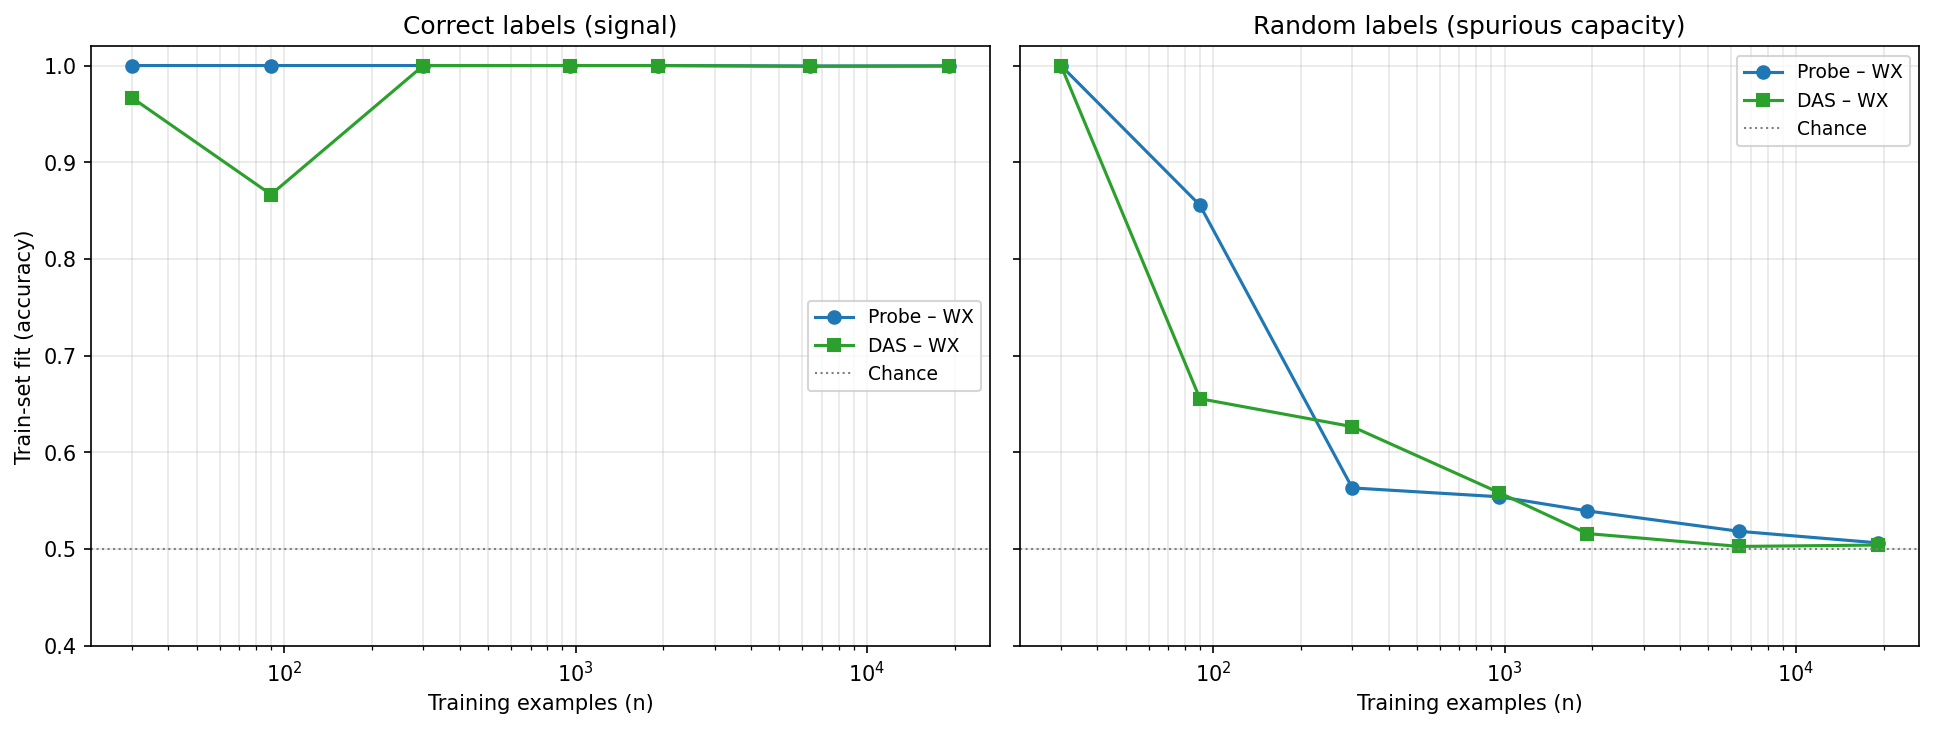
\includegraphics[width=0.6\linewidth]{scaling.png}
\caption{Train-set fit vs.\ number of training examples $n$, for the diagnostic probe
and linear DAS, on correct labels (signal, solid) and a fixed random relabelling
(spurious capacity, dashed). Both recover WX on the correct labels; on random labels
both fall from perfect memorisation at small $n$ toward chance, and DAS's curve lies at
or below the probe's at most sizes (most clearly at $n=90$), indicating lower
spurious-fitting capacity. Single seed.}
\label{fig:scaling}
\end{figure}

We report this as suggestive, not settled. The curves are single-seed and noisy---they
cross once (at $n=300$), and DAS's correct-label fit wobbles at the smallest $n$---so the
gap, which rests largely on the $n=90$ point, needs averaging over seeds before it is
leaned on.

\section*{What this is, and what it is not}

This is a single-seed, single-task, linear-vs-linear comparison, with the ``complexity''
axis instantiated as dataset size rather than probe or alignment-map complexity proper.
Two notes from building it. First, an earlier version measured DAS at chance and we
nearly reported it as a negative result; that was an artefact of a multi-intervention
data generator---the joint intervention produced label-homogeneous batches with no
training signal---not a property of linear alignment, and restricting to a single,
balanced intervention fixed it. Second, causal-probe training must be judged by a
held-out, order-independent evaluation, not the running training accuracy, which drifts
misleadingly. The natural next steps are averaging over seeds and sweeping a genuine
complexity axis (deeper probes; non-linear RevNet alignment maps), the regime in which
the limit results of \citet{pimentel2020information} and \citet{sutter2025nonlinear}
guarantee that both methods must eventually fail.

\small
\bibliographystyle{plainnat}
\bibliography{references}

\end{document}
